\subsection{Task 3: Weakly Connected Component}
\subsubsection{Validity}
We verify the validity of our algorithm in both small and large datasets. For small datasets, we generate several synthetic graph containing a small amount of weakly connected components of different sizes. Then we run our algorithm on this small datasets, the result matches the reality. For large datasets, we use real graph from Konect and SNAP project, we can reproduce the statistics "number of nodes in largest WCC" on their web using our algorithm, which partially demonstrate the correctness of our algorithm .


\subsubsection{Experiment on large datasets}
In this experiment, we run weakly connected component in several datasets of various size (from 100 thousand to 2 million of nodes). In the following, we show the frequency radius plot in log log scale for dataset Email-EuALL (figure \ref{t3:1}), Soc-Sign-Epinions(figure \ref{t3:2},) Trec-wt10g (figure \ref{t3:3}), Google Web Graph (figure \ref{t3:4}), Wiki Talk (figure \ref{t3:5}). 
\begin{figure}[!htbf]
\begin{center}
     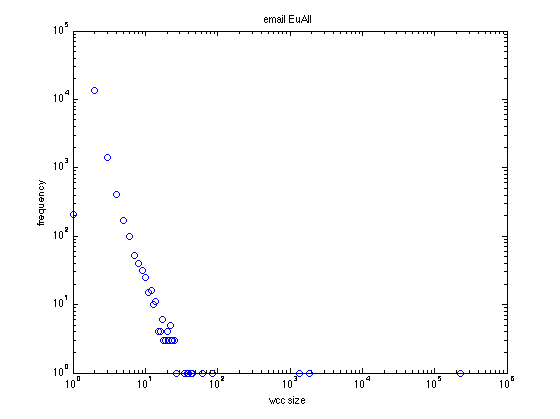
\includegraphics[width=0.8\textwidth]{FIG/t3_email_euall.png} 
\caption{Email-EuAll }
\label{t3:1}
\end{center}
\end{figure}

\begin{figure}[!htbf]
\begin{center}
\begin{tabular}{cc}
     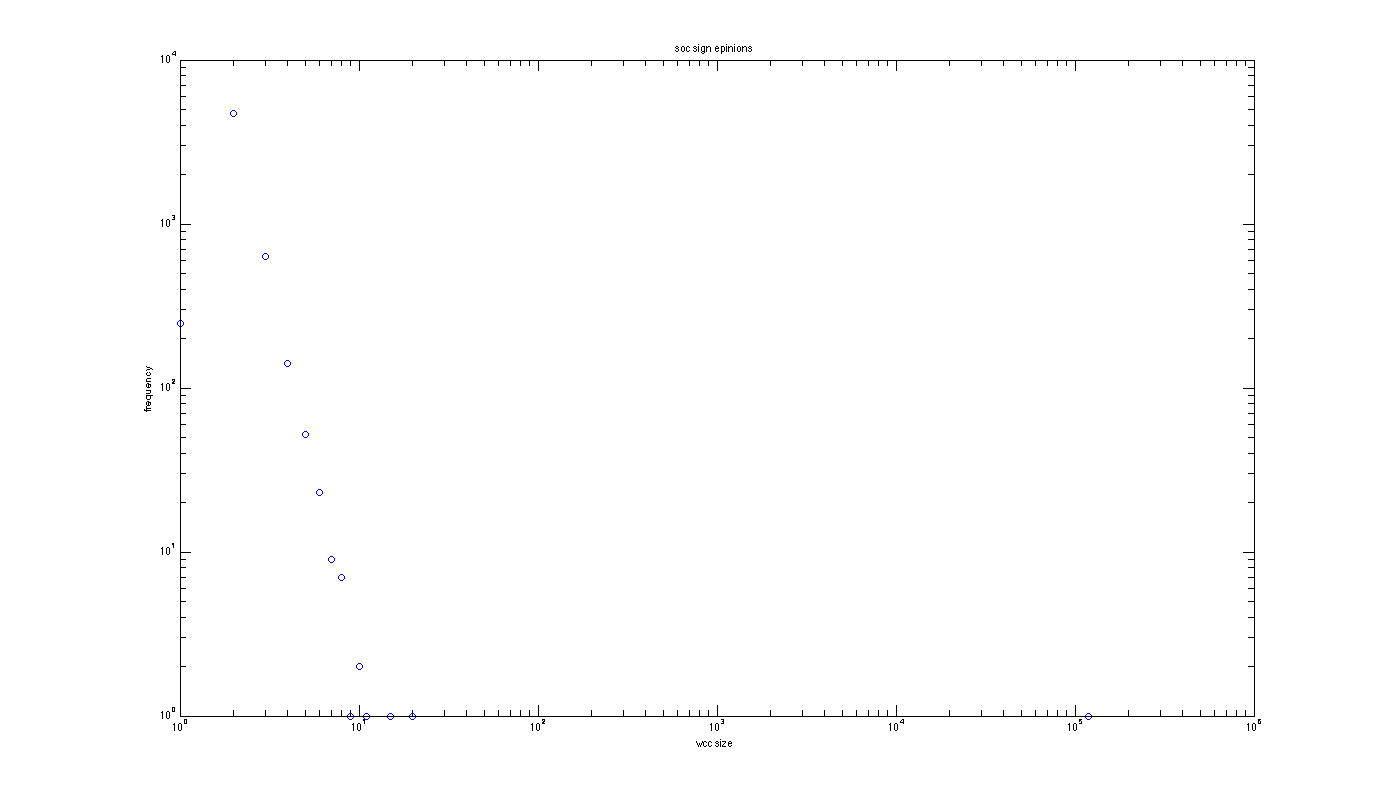
\includegraphics[width=0.8\textwidth]{FIG/t3_soc_sign_epinions.png} 
\end{tabular}
\caption{Soc-Sign-Epinions}
\label{t3:2}
\end{center}
\end{figure}


\begin{figure}[!htbf]
\begin{center}
     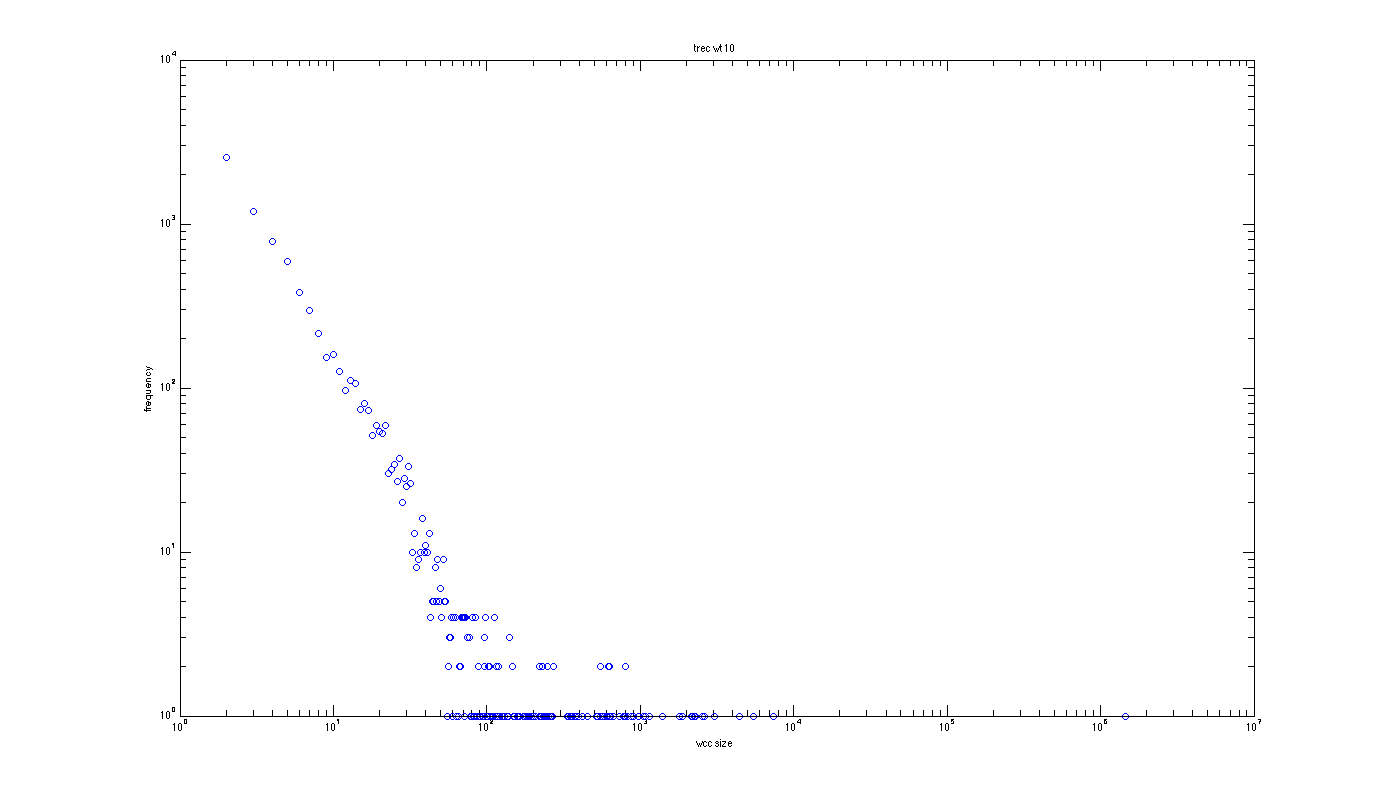
\includegraphics[width=0.8\textwidth]{FIG/t3_trec_wt10.png} 
\caption{Trec-wt10g}
\label{t3:3}
\end{center}
\end{figure}


\begin{figure}[!htbf]
\begin{center}
     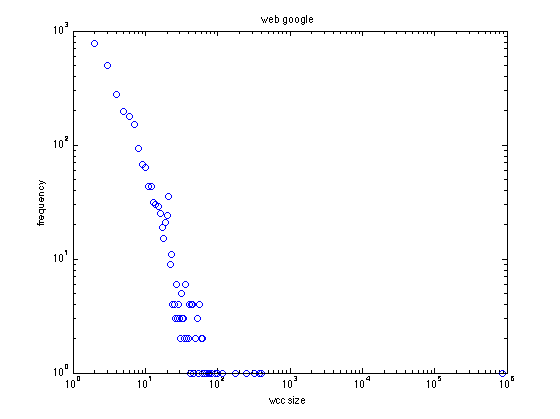
\includegraphics[width=0.8\textwidth]{FIG/t3_web_google.png} 
\caption{Google Web Graph}
\label{t3:4}
\end{center}
\end{figure}


\begin{figure}[!htbf]
\begin{center}
     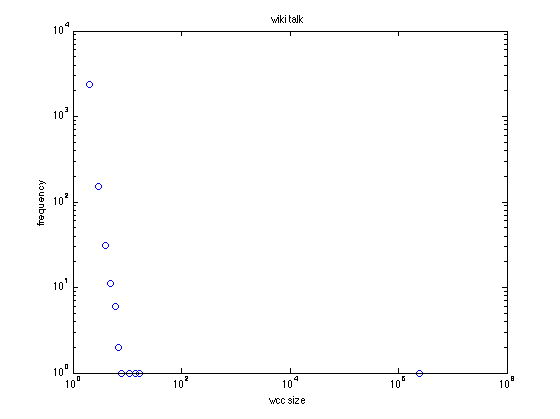
\includegraphics[width=0.8\textwidth]{FIG/t3_wiki_talk.png} 
\caption{Wiki Talk}
\label{t3:5}
\end{center}
\end{figure}

We also run our algorithm in two large connected graphs(com-Youtube and com-amazon), some statistics are presented in table \ref{tbl:wcc}
\begin{table}[!htbf]
\caption{Weakly Connected Component Run Result}
\begin{center}
\begin{tabular}{|c|c|c|c|c|}
\hline \hline
graph & number of nodes & number of edges & number of wcc & nodes in largest wcc \\
\hline
com-Youtube & 1134890 & 2987624 & 1 & 1134890 \\
web-Google & 875713 & 5105039 & 	2746 &  855802 \\ 
com-Amazon & 334863 & 2987624 & 1 & 1134890 \\
email-EuAll & 265214 & 420045 & 15836 & 224832 \\
wiki-talk & 2394385 & 5021410  & 2555  & 2388953 \\
soc-sign-epinions & 131828  & 841372  & 5816 & 119130 \\
trec wt10g & 1601787  & 8063026  & 7955 & 1458316 \\
\hline
\end{tabular}
\end{center}
\label{tbl:wcc}
\end{table}%

 
\subsubsection{Observation}
1. From the log-log scale frequency-size plot, we find that generally frequency-size follows the power law. Connected components of small sizes tend to occur more often those of larger sizes.

2. In all the plots, there is a giant connected component that contains the majority of nodes in the graph. This is a characteristic that almost all large graphs share, for example, in the yahoo web graph, there is also a giant connected component. 




